\section{Good Programming Practices}
\label{research:GoodProgrammingPractices}
\textbf{Source:} \cite{pruimFosteringBetterCoding2023}

\subsection*{Key takeaways:}
\begin{itemize}
    \item "It is easier to notice and fix errors in well-written code. "
    \item "It is easier and more efficient to learn good coding practices as one learns to program than to unlearn bad habits later."
    \item Adding whitespace / splitting processes into multiple steps is not a sign of a bad programmer but one who programs logically
\end{itemize}

\subsection*{4 C's:}
\begin{enumerate}
    \item \textbf{Clarity} - "Code should be easy to read and understand, even for someone who is not the original author."
    \item \textbf{Correctness} - "Code should do what it is intended to do, without errors or bugs."
    \item \textbf{Containment} - "Code should be modular and self-contained, making it easy to reuse and maintain."
    \item \textbf{Consistency} - "Code should follow a consistent style and structure, making it easier to read and understand."
\end{enumerate}


\subsection*{Top 10 list:}
\begin{enumerate}
	\item Choose clear variable names
	\item  Follow style guides - note: need to create one
	\item  Create documents using tools that support reproducible workflows - note: need to make my software compatible with copy/paste from other tools such as word etc 
	\item  Select a coherent and minimal yet powerful toolkit for code
	\item  Don't repeat yourself, use functions!!!!
	\item  Take advantage of functional programming styles
	\item  Employ consistency checks
	\item  Learn to debug effectively 
	\item  Use version control!!! - note: for final artifact will need to use a tool like git rather than the current incremental name system I am currently using
	\item  Use a code formatter - note: need to find a formatter for Visual Studio Code
\end{enumerate}

\begin{figure}[H]
\centering
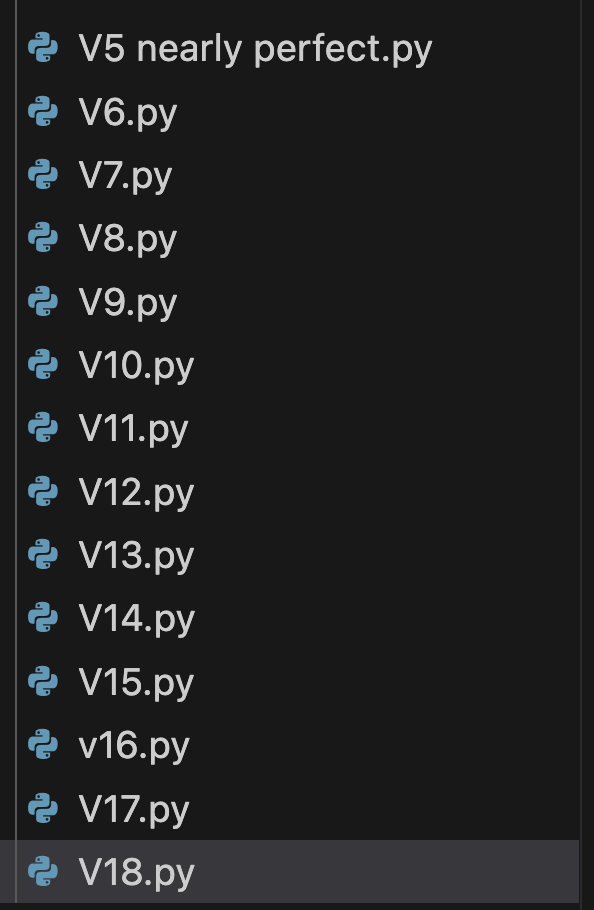
\includegraphics[width=0.4\textwidth]{Research/11_GoodProgrammingPractices/media/bad.png}
\caption{Example of my current (poor) System of version control}
\end{figure}

to rectify this I will need to use a version control system such as git, this will allow me to keep track of changes and revert to previous versions if necessary. 